\documentclass[a4paper,11pt]{article}

% -------------------------------------------------
% Packages
% -------------------------------------------------
\usepackage{polyglossia}
\setmainlanguage{italian}
\usepackage{fontspec}

\usepackage{geometry}
\geometry{
    left=2.5cm,
    right=2.5cm,
    top=2.5cm,
    bottom=2.5cm
}

\usepackage[hidelinks]{hyperref}
\usepackage{graphicx}
\usepackage{listings}
\usepackage{xcolor}
\usepackage{fancyhdr}
\usepackage{titlesec}
\usepackage{graphicx}
\usepackage{minted}
\usepackage{hyperref}
\usepackage{hyperref}


% -------------------------------------------------
% Style
% -------------------------------------------------

\pagestyle{fancy}
\fancyhf{}
\fancyhead[L]{Progetto Bomberman}
\fancyhead[R]{Relazione tecnica}
\fancyfoot[C]{\thepage}

\titleformat{\section}
{\Large\bfseries}
{\thesection}{1em}{}

\titleformat{\subsection}
{\large\bfseries}
{\thesubsection}{1em}{}

\lstset{
    basicstyle=\ttfamily\small,
    breaklines=true,
    frame=single
}

\usemintedstyle{colorful}

\newminted{cpp}{
  frame=lines,
  bgcolor=gray!5,
  fontsize=\small,
  linenos,
  breaklines
}

\setlength{\headheight}{14pt}
\setlength{\parindent}{0pt}
\setlength{\parskip}{6pt}

% -------------------------------------------------
% Document
% -------------------------------------------------

\begin{document}

\begin{titlepage}

\centering

\vspace*{2cm}

{\Huge\bfseries Progetto Bomberman\\[0.5cm]}

{\Large Relazione tecnica}

\vspace{1.5cm}

{\large
Corso di Programmazione\\
Anno accademico 2025/2026
}

\vfill

{\large
Andrea Manzo \\
Tommaso Lissandrin \\
Alessandro Godani
}

\vfill

{\large
Università di Bologna
}

\end{titlepage}


\tableofcontents
\newpage


% -------------------------------------------------

\section{Introduzione}

Il progetto consiste nella realizzazione di una versione testuale del videogioco
\textit{Bomberman}, sviluppata in linguaggio C++ mediante l'utilizzo della
libreria \texttt{ncurses}. L'obiettivo principale è stato applicare in modo
concreto i principi della programmazione orientata agli oggetti, permettendo la
progettazione di un'architettura modulare.

Il gioco riproduce le meccaniche fondamentali del titolo originale: il giocatore
deve attraversare una sequenza di livelli, posizionare bombe strategicamente,
eliminare i nemici presenti nella mappa e raggiungere il termine della partita
ottenendo il punteggio più alto possibile.

La componente grafica è stata implementata tramite una Text User Interface (TUI)
all'interno del terminale, sfruttando la libreria \texttt{ncurses}. Nonostante
i vincoli imposti dall'ambiente testuale, è stato adottato l'utilizzo di una
palette di colori estesa e caratteri Unicode UTF-8, con l'obiettivo di ottenere
una rappresentazione visiva più chiara e strutturata rispetto al semplice ASCII,
pur mantenendo l'esecuzione interamente in ambiente terminale.

Il progetto è stato sviluppato in gruppo, con una suddivisione iniziale delle
responsabilità tra le varie componenti del sistema. Durante la fase iniziale è stato
tuttavia mantenuto un forte livello di collaborazione diretta, con sessioni di
sviluppo condivise e discussione congiunta dell'architettura, al fine di
definire un'impostazione coerente prima della separazione effettiva dei moduli.
Nelle fasi successive, il lavoro è stato progressivamente distribuito in modo
più autonomo, mantenendo comunque un'integrazione continua tra le parti sviluppate.

\begin{figure}[h]
    \centering
    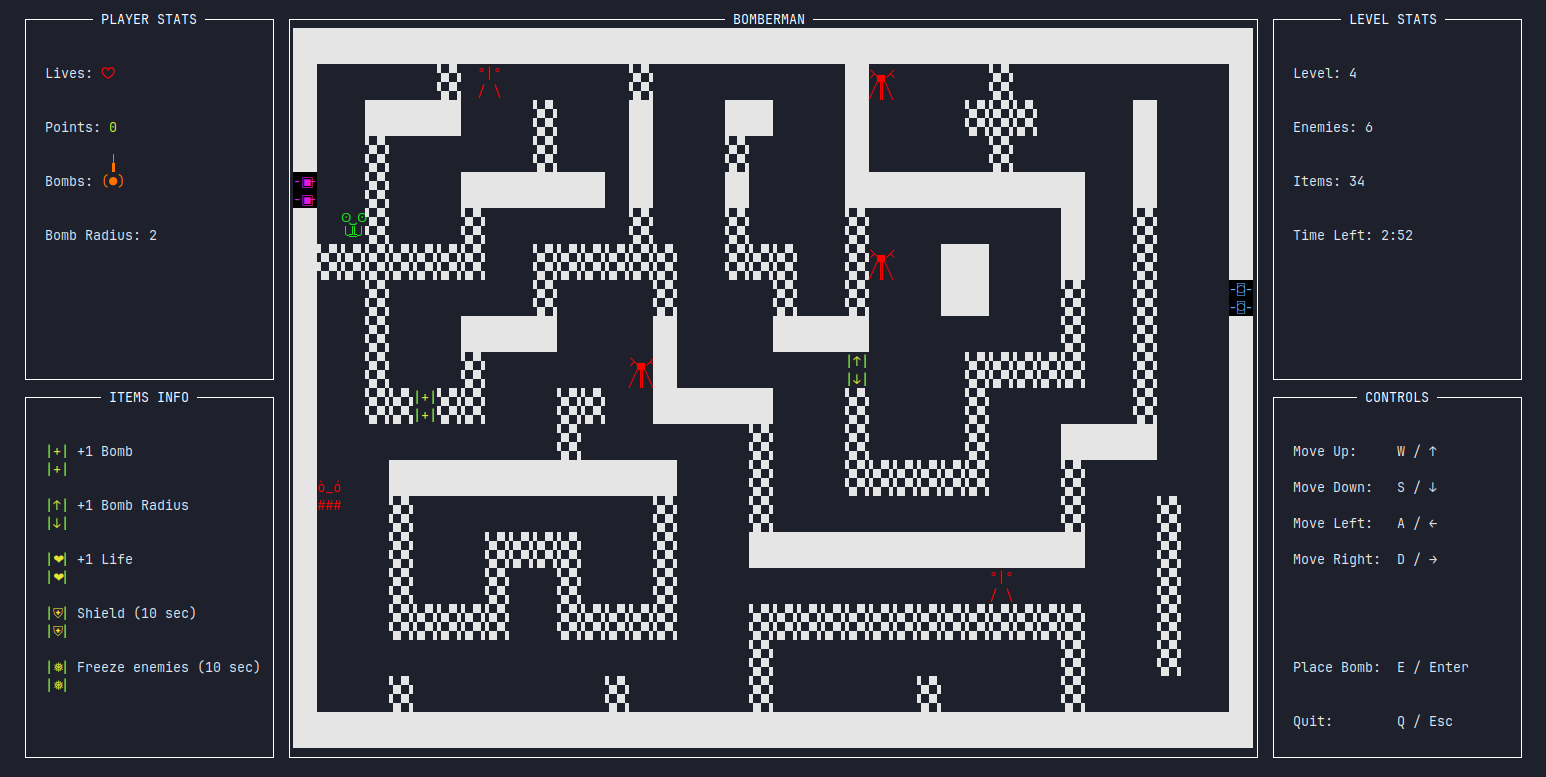
\includegraphics[width=0.8\textwidth]{esempio_schermata.png}
    \caption{Esempio di schermata di gioco}
    \label{fig:gameplay}
\end{figure}

\section{Organizzazione del progetto}

Il progetto è stato organizzato seguendo una struttura modulare, separando le
componenti logiche del gioco dalla parte grafica e dalle funzionalità di
supporto.

L'architettura si basa su una chiara separazione tra le entità di gioco e il
componente responsabile della gestione del livello. Le entità principali
(Player, Enemy, Bomb, Item) rappresentano oggetti autonomi che mantengono
solamente il proprio stato interno e non hanno conoscenza diretta degli altri
elementi presenti nella mappa.

La gestione delle interazioni tra le entità e dell'evoluzione dello stato di
gioco è centralizzata nella classe \texttt{Level}, che rappresenta il nucleo
del gameplay insieme alla classe \texttt{Game}. 
Questa scelta evita dipendenze dirette tra le classi e consente
di mantenere le entità indipendenti tra loro, demandando al livello la
risoluzione di collisioni ed effetti.

\subsection{Classi principali}

Le principali classi del progetto sono:

\begin{itemize}

    \item \textbf{Game}: rappresenta una singola partita. Gestisce il ciclo
    principale di gioco relativo ai livelli, occupandosi della creazione e
    gestione del livello corrente, dell'aggiornamento dello stato del giocatore
    e della progressione tra i livelli.

    \item \textbf{Level}: è il componente centrale del gameplay. Contiene la
    rappresentazione della mappa e gestisce l'aggiornamento dello stato del
    livello.

    La classe si occupa della gestione della griglia, del caricamento della
    configurazione del livello, del disegno degli elementi e della gestione
    delle interazioni tra entità, come le collisioni, le esplosioni delle bombe
    e il raccoglimento degli items.

    \item \textbf{LevelList}: è il componente che gestisce l'insieme dei livelli, implementato 
    come lista bidirezionale, in modo da gestire al meglio il passaggio da un livello all'altro
    e la rimozione dei livelli completati.

    \item \textbf{Player}: rappresenta il personaggio controllato dall'utente.
    Mantiene lo stato del giocatore, come posizione, vite, bombe, e gestisce gli 
    effetti degli items.

    \item \textbf{Enemy}: rappresenta i nemici presenti nella mappa. Ci sono tre
    diversi tipi di nemico e ognuno mantiene il proprio stato e comportamento.

    \item \textbf{Bomb}: rappresenta una bomba piazzata dal giocatore (o da un nemico).
    Contiene informazioni sul proprio stato, come posizione e tempo residuo
    prima dell'esplosione. Gli effetti dell'esplosione vengono gestiti dal
    livello.

    \item \textbf{Item}: rappresenta gli oggetti ottenibili durante la partita.
    L'oggetto conserva le proprie informazioni e può essere raccolto dal player
    per ottenere abilità temporanee o miglioramenti permanenti.

    \item \textbf{Menu}: gestisce la schermata iniziale del gioco e permette
    all'utente di selezionare le diverse opzioni disponibili.

    \item \textbf{ScoreBoard}: si occupa della gestione della classifica,
    leggendo e scrivendo i punteggi su file in modo persistente tra diverse
    esecuzioni del programma.

\end{itemize}


\subsection{Gestione della grafica tramite modulo NcWrapper}

Per evitare l'utilizzo diretto della libreria \texttt{ncurses} all'interno delle componenti di gameplay, 
è stato introdotto un modulo di astrazione denominato \texttt{NcWrapper}. 
Tale modulo incapsula le funzionalità legate alla gestione del terminale e della rappresentazione grafica, 
fornendo un'interfaccia indipendente dalla libreria sottostante.

Il modulo \texttt{NcWrapper} è organizzato in più componenti specializzate:

\begin{itemize}
    \item \textbf{NcFunctions}: contiene le funzioni di inizializzazione e gestione del terminale, 
    come avvio e terminazione della modalità grafica, controllo delle dimensioni del terminale e 
    gestione dell'input;
    
    \item \textbf{NcTypes}: definisce i tipi fondamentali utilizzati dal modulo, tra cui 
    enumerazioni per input (\texttt{Key}), gestione dei colori (\texttt{Color}) e primitive geometriche come \texttt{Point};
    
    \item \textbf{Sprite2x3}: rappresenta l'unità base di rendering grafico. 
    Ogni sprite è definito come una matrice 2x3 di caratteri testuali associata a informazioni di colore 
    e background, permettendo la rappresentazione di elementi di gioco in forma stilizzata;
    
    \item \textbf{Window}: implementa una finestra logica basata su \texttt{ncurses WINDOW}, 
    fornendo primitive di disegno ad alto livello e incapsulando la gestione delle operazioni di rendering.
\end{itemize}

\begin{figure}[h]
    \centering
    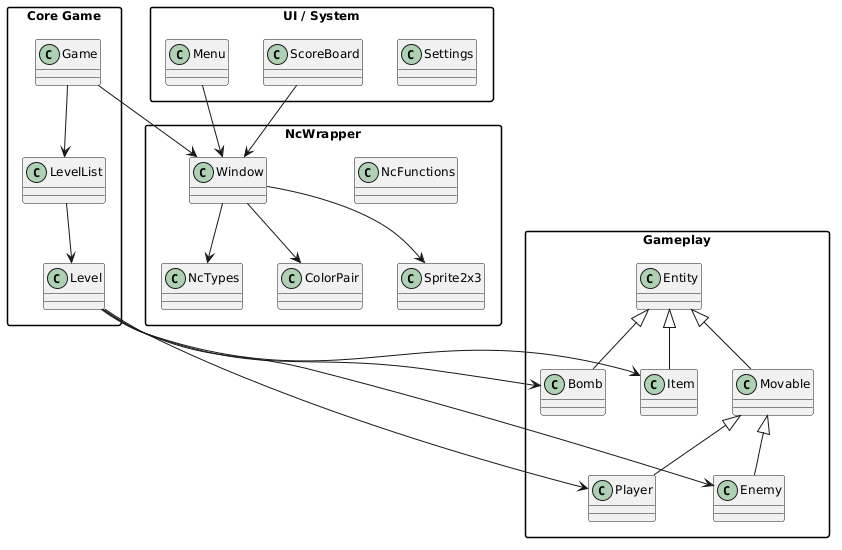
\includegraphics[width=0.8\textwidth]{diagramma.png}
    \caption{Architettura generale del sistema e relazioni tra classi principali}
    \label{fig:architecture}
\end{figure}

La classe \texttt{Window} rappresenta il principale punto di interazione tra il gioco e il sistema di visualizzazione. 
Essa astrae le funzionalità di basso livello della libreria \texttt{ncurses}, fornendo operazioni come:

\begin{itemize}
    \item disegno di sprite tramite \texttt{Sprite2x3};
    \item scrittura di testo con supporto a colori e background;
    \item gestione del titolo e del layout della finestra;
    \item aggiornamento e pulizia del buffer di rendering;
    \item acquisizione dell'input utente in modo contestualizzato.
\end{itemize}

Questa organizzazione consente di separare chiaramente la logica di rendering dalle regole di gioco, 
riducendo la dipendenza diretta del codice applicativo dalla libreria \texttt{ncurses}. 
Le componenti di gameplay interagiscono esclusivamente con le astrazioni fornite dal modulo \texttt{NcWrapper}, 
senza conoscere i dettagli implementativi del sistema di visualizzazione, permettendo anche una
maggiore portabilità del codice, grazie alla possibilità di sostituire il backend grafico senza modifiche alla logica di gioco.

In questo modo, il sistema di rendering viene trattato come un sottosistema indipendente, 
che espone primitive coerenti e riutilizzabili, mentre le classi di gioco operano esclusivamente 
su concetti ad alto livello senza dipendere dai dettagli della libreria sottostante.


\subsection{Gestione delle mappe e della classifica}

Il progetto adotta un approccio basato su persistenza tramite file di testo per la gestione sia delle mappe 
di gioco sia della classifica dei punteggi. Questa scelta consente di separare i dati di configurazione e stato 
dal codice eseguibile, facilitando l'estendibilità del sistema e la modifica dei contenuti senza necessità di ricompilazione.

\paragraph{Gestione delle mappe}

Le mappe di gioco sono memorizzate in file di testo strutturati, in cui ogni carattere rappresenta un elemento 
della griglia di gioco. Il caricamento avviene all'interno del costruttore della classe \texttt{Level}, 
che esegue il parsing sequenziale del file e la costruzione della rappresentazione interna della mappa.

Durante la lettura, ogni carattere viene interpretato secondo una codifica predefinita:

\begin{itemize}
    \item \texttt{X}: muro solido non attraversabile;
    \item \texttt{\#}: muro distruttibile;
    \item \texttt{O}: porta di accesso al livello successivo;
    \item \texttt{P}: porta di ritorno al livello precedente;
    \item \texttt{1,2,3}: tipologie differenti di nemici con posizionamento iniziale;
    \item altri caratteri: celle vuote.
\end{itemize}

Il parser mantiene un controllo rigoroso sulla validità strutturale del file, 
verificando la consistenza delle dimensioni rispetto ai limiti definiti da \texttt{Settings}. 

Oltre alla costruzione della griglia, il caricamento della mappa inizializza anche le entità dinamiche 
(nemici e oggetti), derivandole direttamente dalla configurazione testuale. 

\paragraph{Gestione della classifica}

La classifica dei punteggi è implementata tramite una struttura dati dinamica basata su lista concatenata ordinata. 
I dati vengono persistiti su file di testo, permettendo il mantenimento delle informazioni tra diverse esecuzioni del programma.

All'avvio del sistema, il file della classifica viene letto sequenzialmente e nel caso in cui 
il file non esista, viene creato automaticamente un file vuoto, garantendo la corretta inizializzazione del sistema di persistenza.

I dati letti vengono inseriti in una lista ordinata in modo decrescente rispetto al punteggio. 
L'inserimento mantiene sempre la proprietà di ordinamento senza necessità di operazioni di riordinamento globali, 
ottimizzando l'aggiornamento incrementale della struttura.

Alla chiusura del programma il file viene aggiornato con le nuove modifiche della classifica.

\section{Suddivisione del lavoro}

Lo sviluppo del progetto è stato organizzato secondo una suddivisione delle responsabilità tra i membri del gruppo. 
Nonostante tale ripartizione, la fase iniziale è stata caratterizzata da un'attività di progettazione congiunta, 
in particolare per la definizione delle interfacce pubbliche delle classi (\texttt{.hpp}), 
con l'obiettivo di stabilire un'API comune coerente su cui basare l'intero sistema. 
Tale impostazione è stata successivamente estesa e raffinata in modo incrementale durante l'implementazione.

La distribuzione delle principali responsabilità è riassunta nella Tabella~\ref{tab:suddivisione}.

\bigskip

\begin{table}[h]
\centering
\begin{tabular}{|l|l|}
\hline
\textbf{Membro} & \textbf{Componenti sviluppate} \\
\hline
Andrea Manzo & NcWrapper, Bomb, Game \\
\hline
Tommaso Lissandrin & Item, Player, LevelList, ScoreBoard \\
\hline
Alessandro Godani & Enemy, Level (costruttore e gestione mappa), Menu, mappe di livello \\
\hline
\end{tabular}
\caption{Suddivisione delle responsabilità tra i membri del gruppo}
\label{tab:suddivisione}
\end{table}

Nonostante la suddivisione formale, lo sviluppo di diverse componenti è avvenuto in modo condiviso o iterativo. 
In particolare, la classe \texttt{Level} rappresenta un caso di collaborazione trasversale: 
ad esempio, le funzioni relative alla gestione delle bombe sono state implementate principalmente da Andrea Manzo, 
mentre le logiche relative ai nemici sono state sviluppate da Alessandro Godani.

Le classi non incluse nella tabella sono da considerarsi ausiliarie o realizzate in una fase iniziale 
di progettazione collaborativa.

\section{Utilizzo degli LLM}

Durante lo sviluppo del progetto sono stati utilizzati Large Language Models
come strumenti di supporto alla progettazione e al miglioramento del codice.
Gli LLM non sono stati utilizzati per generare automaticamente il progetto,
ma principalmente per analizzare soluzioni esistenti, proporre refactoring e
migliorare la struttura del codice.

Ogni suggerimento è stato valutato manualmente e applicato solamente quando
compatibile con l'architettura scelta. Di seguito più in dettaglio l'utilizzo 
da parte di ogni componente del gruppo.

\subsection{Andrea Manzo}

L'utilizzo degli LLM nella mia parte di sviluppo è avvenuto con modalità differenti in base al tipo di problematica affrontata. 
In alcuni casi sono stati utilizzati come supporto alla comprensione di aspetti tecnici specifici, 
ad esempio per approfondire il funzionamento della libreria \texttt{ncurses} o individuare possibili soluzioni 
a problemi legati alla gestione grafica. 

In altri contesti il loro utilizzo è stato maggiormente orientato alla progettazione e alla valutazione di scelte architetturali, fornendo possibili strategie di riorganizzazione del codice e aiutando a individuare una suddivisione più efficace delle responsabilità tra componenti.

Infine, per alcune parti caratterizzate da codice ripetitivo e poco significativo dal punto di vista logico, gli LLM sono stati utilizzati come supporto diretto alla scrittura del codice, velocizzando attività manuali come la generazione di elementi dell'interfaccia grafica e la gestione di numerosi dettagli implementativi.

In tutti i casi il codice e i suggerimenti prodotti dal modello sono stati considerati come proposte da analizzare e verificare, applicandoli solamente quando compatibili con l'architettura e le scelte progettuali del progetto.
\subsubsection{Refactoring della gestione delle bombe}

Un utilizzo significativo degli LLM ha riguardato la revisione della logica di gestione delle bombe e delle esplosioni all'interno della classe \texttt{Level}. 
La problematica iniziale era legata alla presenza di diverse responsabilità concentrate nello stesso componente: gestione dello stato della bomba, temporizzazione, calcolo delle celle coinvolte nell'esplosione, applicazione degli effetti sulle entità e visualizzazione dell'esplosione.

Gli LLM sono stati utilizzati come supporto durante la fase di analisi del codice esistente, chiedendo valutazioni sulla suddivisione delle responsabilità e su possibili strategie di refactoring. 
In particolare, è stato analizzato se fosse opportuno spostare parte della logica dalla classe \texttt{Level} verso componenti più specifici, mantenendo comunque un equilibrio tra modularità e semplicità architetturale.

Il suggerimento principale emerso è stato quello di distinguere maggiormente le diverse fasi del ciclo di vita della bomba:
\begin{itemize}
    \item gestione temporale e aggiornamento dello stato della bomba;
    \item determinazione delle celle raggiunte dall'esplosione;
    \item applicazione degli effetti su mappa e giocatore;
    \item separazione della fase di rendering dalla logica di gioco.
\end{itemize}

La proposta è stata valutata e adattata all'architettura già presente nel progetto. 
Non è stata introdotta una completa separazione della logica in nuove classi, poiché \texttt{Level} rappresenta il punto di coordinamento naturale delle interazioni tra le varie entità del gioco. 
È stata invece migliorata la suddivisione interna delle responsabilità tramite funzioni con compiti più specifici.

La revisione ha portato a una distinzione più chiara tra:
\begin{itemize}
    \item \texttt{Bomb::update()}, responsabile dell'aggiornamento dello stato temporale della bomba e dei cambiamenti grafici associati;
    \item \texttt{Level::handleBombs()}, responsabile dell'inserimento della bomba nel flusso di gioco e della gestione del suo ciclo di vita;
    \item funzioni ausiliarie come \texttt{setExplosionCells()} e \texttt{applyExplosion()}, dedicate rispettivamente al calcolo dell'area dell'esplosione e all'applicazione degli effetti sulle entità coinvolte.
\end{itemize}

La struttura finale della gestione delle bombe è quindi suddivisa nelle seguenti funzioni principali:

\begin{minted}[fontsize=\small]{cpp}
void Bomb::update();

void Level::handleBombs(Player& player);

void Level::setExplosionCells(Bomb& bomb);

void Level::applyExplosion(const Bomb& bomb, Player& player);

void Level::drawExplosion(const Bomb& bomb, Nc::Window& window);
\end{minted}

Il risultato finale è una struttura più modulare e leggibile, in cui ogni funzione ha una responsabilità più definita, mantenendo allo stesso tempo il controllo delle interazioni all'interno del livello di gioco.


\subsubsection{Definizione di una palette colori estesa}

Un altro utilizzo degli LLM ha riguardato la gestione dei colori dell'interfaccia grafica basata sulla libreria \texttt{ncurses}. 
La versione iniziale del sistema utilizzava solamente i colori standard messi a disposizione dalla libreria, limitando la possibilità di differenziare visivamente gli elementi presenti nel gioco.

Durante lo sviluppo è emersa quindi la necessità di introdurre una palette più ampia, in modo da poter rappresentare in maniera più chiara oggetti diversi come entità, esplosioni, oggetti ottenibili e componenti dell'interfaccia.

Gli LLM sono stati utilizzati come supporto per analizzare il funzionamento della gestione dei colori in \texttt{ncurses}, in particolare riguardo alla possibilità di definire colori personalizzati tramite la funzione \texttt{init\_color()} e al meccanismo di conversione tra colori applicativi e identificativi interni della libreria.

Un aspetto particolarmente utile è stato l'utilizzo degli LLM per generare automaticamente una prima proposta di palette completa. 
La generazione automatica ha permesso di evitare la scelta manuale di numerosi valori RGB, fornendo una base iniziale successivamente verificata e adattata in base alle esigenze grafiche del progetto.

\begin{minted}[fontsize=\small]{cpp}
init_color(8,  1000, 450, 0);   // Orange
init_color(11, 1000, 400, 700); // Pink
init_color(13, 400, 700, 1000); // Sky
init_color(15, 1000, 800, 200); // Gold
init_color(18, 650, 300, 150);  // Brick
\end{minted}

La soluzione finale adottata consiste nella definizione di una serie di colori personalizzati oltre a quelli standard forniti da \texttt{ncurses}. 
Ogni colore è associato ad un nome significativo tramite l'enumerazione \texttt{Nc::Color}, evitando l'utilizzo diretto degli identificativi numerici della libreria all'interno del codice di gioco.
In questo modo le classi del gameplay possono utilizzare colori descrittivi come \texttt{Orange}, \texttt{Fire} o \texttt{LightGray} senza dipendere direttamente dai valori numerici della libreria grafica.

\begin{minted}[fontsize=\small]{cpp}
short toNcurses(Color c)
...

case Color::Sky:        return 13;
case Color::Purple:     return 14;
case Color::Gold:       return 15;
case Color::Fire:       return 16;
case Color::LightBrown: return 17;
case Color::Brick:      return 18;
\end{minted}


L'intervento ha migliorato la leggibilità del codice e ha reso più semplice l'estensione futura della grafica, permettendo di aggiungere nuovi colori senza modificare la logica delle entità di gioco.

\subsubsection{Supporto alla generazione dei menu laterali nella schermata di gioco}

Un ulteriore utilizzo degli LLM ha riguardato la realizzazione e la gestione della schermata di gioco, in particolare la parte relativa ai menu laterali visualizzati durante una partita.

Questa componente non presentava particolari difficoltà dal punto di vista algoritmico, ma risultava molto lunga e soggetta a errori manuali. 
La costruzione dell'interfaccia richiedeva infatti numerose operazioni ripetitive: scrittura di stringhe, 
scelta delle coordinate corrette, gestione degli spazi tra gli elementi, selezione dei colori...

In questo caso gli LLM sono stati utilizzati principalmente come assistenti nella scrittura del codice. 
L'approccio adottato è stato iterativo: veniva fornita al modello una descrizione della porzione di interfaccia da realizzare, specificando la posizione desiderata degli elementi, le informazioni da mostrare e le convenzioni grafiche utilizzate dal progetto. 
Il codice generato veniva poi analizzato, corretto e integrato manualmente nel programma.

L'utilizzo del modello è risultato particolarmente utile per attività ripetitive che, pur essendo semplici, richiedevano attenzione ai dettagli. 

Questa parte di codice è quella racchiusa nelle funzioni:

\begin{minted}[fontsize=\small]{cpp}
void Game::writeOnMenus();

void Game::writeTimedItems();
\end{minted}

L'intervento degli LLM non ha modificato l'architettura generale del sistema, ma ha permesso di velocizzare una fase di sviluppo caratterizzata da molto codice di collegamento tra logica del gioco e interfaccia grafica. 
Il risultato è stato ottenuto mantenendo comunque una verifica manuale del codice prodotto, necessaria per garantire coerenza con le convenzioni e le scelte progettuali già presenti.

\subsubsection{Considerazioni finali}

In generale, ho trovato l'utilizzo degli LLM particolarmente utile come strumento di affiancamento alla programmazione, soprattutto nelle fasi di sviluppo caratterizzate da codice ripetitivo o da una forte componente implementativa. In questi contesti, il supporto del modello mi ha permesso di ridurre il carico di lavoro manuale e di concentrarmi maggiormente sugli aspetti architetturali e logici del progetto.

Un altro ambito in cui si sono rivelati efficaci riguarda l'individuazione e la risoluzione di bug poco evidenti o difficili da diagnosticare, dove il confronto con il modello mi ha spesso aiutato a considerare casi limite o comportamenti non immediatamente visibili.

Ho trovato particolarmente utile anche l'impiego degli LLM come strumento di confronto con pratiche comuni nello sviluppo software reale, ad esempio per comprendere quali siano le soluzioni più adottate in contesti industriali o quali pattern vengano generalmente preferiti in situazioni simili.

Infine, li ho utilizzati anche in un'ottica di apprendimento personale, per approfondire aspetti specifici del linguaggio C++ 
o del funzionamento di determinate librerie, soprattutto quando si trattava di dettagli tecnici o difficili da interpretare in modo autonomo.

\subsection{Tommaso Lissandrin}

Durante lo sviluppo del progetto ho utilizzato i modelli di linguaggio in diversi contesti, considerandoli sempre come uno strumento integrativo, utile specialmente per la possibilità di riassumere rapidamente più fonti di ricerca.
\subsubsection{Approfondimento del linguaggio C++}

I casi più significativi di utilizzo dei modelli di linguaggio riguardano l'apprendimento, o l'approfondimento, di nuovi costrutti del linguaggio C++ e di alcune librerie.

Tra questi, per la gestione della ScoreBoard, ho usufruito di diverse funzioni presenti nella libreria fstream, a me totalmente estranea.
I modelli di linguaggio mi hanno fornito una panoramica generale sulle funzioni principali della libreria, includendo sintassi corretta e gestione di possibili eccezioni per ognuna di esse.

La seguente porzione di codice fa parte del costruttore della ScoreBoard:
\begin{minted}[fontsize=\small]{cpp}
ScoreBoard::ScoreBoard(const char* filePath)
{
  // tentativo di lettura dal file state/scoreboard.txt
  std::ifstream file{ filePath };

  if (!file) // qualora il file non esistesse, verrebbe creato all'interno del corpo dell'if
  {
    std::ofstream create(filePath); // crea file vuoto
    create.close();

    file.open(filePath); // riapre in lettura
  }
  ...
}
\end{minted}

Ho trovato che lo studio della libreria fosse più conveniente ed approcciabile in questo modo, per via della possibilità di fare domande e chiedere ulteriori esempi qualora non trovassi chiaro il funzionamento delle funzioni.
\subsubsection{Ottimizzazione e correzione del codice}

Un utilizzo minore dei modelli di linguaggio è stato fatto per svolgere controlli più accurati su funzioni da me implementate, specialmente per la gestione di strutture dinamiche, così da evitare casi di memory leak difficili da individuare.

La seguente funzione, utilizzata per inserire ordinatamente i giocatori nella classifica (gestita come una lista), è stata controllata anche da un modello di linguaggio:
\begin{minted}[fontsize=\small]{cpp}
// push di un elemento in ordine decrescente di punteggio
void ScoreBoard::pushOrderly(const char* playerName, const int score) 
{
  Node* foo = new Node;
  strncpy(foo -> playerName, stringPolish(playerName), s_maxNameLenght - 1);
  foo -> playerName[s_maxNameLenght - 1] = '\0'; // assicuro che l'ultimo char sia nullchar
  foo -> score = score;
  m_size++;
  
  if (m_head == nullptr)
  {  
    m_head = foo;
  }
  else if (m_head -> score < score)
  {
    foo -> next = m_head;
    m_head = foo;
  }
  else
  {
    Node* check = m_head;
    while (check -> next != nullptr)
    {
      if ((check -> next) -> score < score)
      {
        foo -> next = check -> next;
        check -> next = foo;
        return;
      }
      check = check -> next;
    }
    check -> next = foo;
  }
}
\end{minted}

Tuttavia ho cercato sempre di limitare questa pratica, in quanto credo che la comprensione ed il collaudo di ciò che si implementi sia una una capacità essenziale per ogni sviluppatore. 

\subsubsection{Tecniche comuni di approccio a problemi noti}

I modelli di linguaggio sono stati utili anche nel suggerire tecniche di approccio comuni in determinati contesti.

Un esempio di ciò si ha nella funzione di controllo delle collisioni tra entità contenuta nella classe Entity:
\begin{minted}[fontsize=\small]{cpp}
bool Entity::collide(const Entity& other) const
{
  int width{ Settings::entityWidth };
  int height{ Settings::entityHeight };
  
  return m_x + width > other.m_x && m_y + height > other.m_y &&
         m_x < other.m_x + width && m_y < other.m_y + height;
}
\end{minted}
L'algoritmo utilizzato è noto come AABB Collision Detection (Axis-Alligned Bounding Box), mi è stato suggerito dai modelli di linguaggio poiché comune nello sviluppo 2D e molto leggero.
Si basa sull'assunzione che le entità possano essere racchiuse in rettangoli immaginari, di cui si vada a controllare la possibile sovrapposizione tramite la condizione di ritorno.

\subsubsection{Considerazioni finali}

Ritengo che i grandi modelli di linguaggio siano stati uno strumento utile per integrare e velocizzare il lavoro.
Sono stati molto efficaci quando fosse necessario fare considerazioni generali, riguardanti strutture dati note e problemi comuni, ma si sono rivelati limitati nelle situazioni in cui il codice a loro fornito fosse profondamente legato all'architettura del progetto.

\subsection{Alessandro Godani}

Il mio utilizzo degli LLM durante lo sviluppo del progetto si è articolato in modalità
diverse a seconda della natura del problema affrontato. In certi casi sono stati
impiegati come strumenti di apprendimento, per acquisire rapidamente la padronanza
di una libreria poco familiare o come interlocutori tecnici,utili per discutere
scelte architetturali e valutarne le implicazioni prima di procedere all'implementazione. 
In altri ancora, il supporto è stato più operativo, orientato alla risoluzione di 
problemi concreti emersi durante lo sviluppo.

In tutti i casi il codice e le spiegazioni prodotte dal modello sono stati trattati
come punto di partenza da analizzare e validare criticamente, non come soluzioni
definitive da applicare direttamente.

\subsubsection{Comprensione della libreria \texttt{ncurses} e struttura del gioco}

Uno dei primi utilizzi degli LLM ha riguardato la comprensione della libreria
\texttt{ncurses} e la struttura generale di un gioco basato su TUI.

Non avendo esperienza pregressa con la libreria, ho utilizzato il modello come
strumento di introduzione guidata, chiedendo spiegazioni sulle funzioni principali
e sul loro utilizzo tipico in un contesto di gioco. 

\subsubsection{Gestione del movimento dei nemici}
 
Una delle problematiche più significative che ho affrontato riguarda la progettazione
del sistema di movimento dei nemici. La difficoltà principale consisteva nel definire
un'architettura in cui le entità non dovessero conoscere direttamente la mappa, ma
il controllo delle collisioni fosse comunque centralizzato.
 
La soluzione adottata, discussa con il modello, è stata quella di delegare l'intera
logica di spostamento alla funzione \texttt{Level::moveEnemies()}, che ha piena
visibilità sulla griglia e su tutte le entità presenti. L'entità nemica espone
solamente operazioni sul proprio stato interno: \texttt{shouldMove()}, \texttt{move()},
\texttt{getDirection()} e \texttt{setDirection()}.
 
La funzione \texttt{Enemy::move()} si limita a invocare \texttt{Movable::move()}
passando la propria direzione corrente, senza sapere nulla della mappa:
 
\begin{minted}[fontsize=\small]{cpp}
void Enemy::move() { Movable::move(m_direction); }
\end{minted}
 
Tutta la logica di collisione e cambio di direzione è invece responsabilità di
\texttt{Level::moveEnemies()}. Dopo aver chiamato \texttt{enemy.move()}, il livello
verifica se il nemico è finito su una cella proibita (muro o bomba del giocatore).
In caso affermativo inverte la direzione, riesegue il movimento, e sceglie una nuova
direzione casuale diversa dalla precedente:
 
\begin{minted}[fontsize=\small]{cpp}
if (!enemy.shouldMove()) continue;
 
enemy.move();
 
bool bombCollide = false;
for (int k = 0; k < m_bombsSize && !bombCollide; k++) {
    Bomb& bomb = m_bombs[k];
    if (bomb.getType() == Bomb::Type::Enemy) continue;
    if (bomb.getStatus() == Bomb::Status::Placed && bomb.collide(enemy))
        bombCollide = true;
}
 
if (checkWallCollision(enemy) || bombCollide) {
    Direction prevDir = enemy.getDirection();
    enemy.setDirection(getOppositeDir(prevDir));
    enemy.move();
 
    do {
        enemy.setDirection(static_cast<Direction>(Random::get(1, 4)));
    } while (enemy.getDirection() == prevDir);
}
\end{minted}
 
Si noti che le bombe di tipo \texttt{Bomb::Type::Enemy} vengono escluse dal
controllo: i nemici non vengono bloccati dalle proprie bombe, ma solo da quelle del
giocatore. Infine, per i livelli avanzati (dal quarto in poi), i nemici di tipo
\texttt{First\_Enemy} hanno un comportamento imprevedibile aggiuntivo, attivato tramite
il flag \texttt{surprise}, che con una certa probabilità causa un cambio di direzione
casuale ad ogni frame indipendentemente dalle collisioni:
 
\begin{minted}[fontsize=\small]{cpp}
if (enemy.getSurpriseStatus()) {
    if (Random::get(0, 50) < 10)
        enemy.setDirection(static_cast<Direction>(Random::get(1, 4)));
}
\end{minted}


\subsubsection{Creazione degli sprite dei nemici in UTF-8}
 
Un ulteriore utilizzo degli LLM ha riguardato la creazione degli sprite testuali
per i nemici. Nel progetto, la rappresentazione grafica delle entità è basata sulla
classe \texttt{Nc::Sprite2x3}, che descrive un'area di
\textbf{2 righe per 3 colonne} di caratteri, con associazioni di colore e background.
Ogni sprite è definito da un piccolo blocco di caratteri testuali che viene
stampato nel terminale nella posizione corrispondente all'entità.
 
Il problema principale era trovare combinazioni di caratteri Unicode che, nella
griglia 2$\times$3 del terminale, producessero una figura
riconoscibile come un personaggio nemico. La scelta dei caratteri giusti
richiede una certa conoscenza del repertorio Unicode e della loro resa effettiva nel
terminale.
 
Ho utilizzato il modello per esplorare le opzioni disponibili, richiedendo caratteri
adatti a comporre figure stilizzate all'interno del vincolo di soli 6 celle. Il
processo è stato iterativo: il modello proponeva combinazioni, che venivano testate
nel terminale e valutate rispetto alla leggibilità visiva e alla coerenza grafica con
il resto del gioco. Il contributo del modello in questa fase è stato prevalentemente
esplorativo, permettendo di considerare un repertorio più ampio di simboli Unicode
rispetto a quanto sarebbe stato possibile ricercando manualmente.
 
\subsubsection{Logica delle bombe del \texttt{ThirdEnemy}}
 
Un utilizzo particolarmente significativo degli LLM ha riguardato la progettazione
della logica relativa alle bombe del terzo tipo di nemico (\texttt{ThirdEnemy}).
A differenza dei primi due tipi, questo nemico ha la capacità di piazzare bombe
autonomamente, il che ha introdotto la necessità di decidere come strutturare questa
funzionalità in modo coerente con l'architettura esistente.
 
La prima questione riguardava \textit{dove collocare} il codice di piazzamento.
Il modello ha confermato che la scelta più coerente era inserirlo in
\texttt{Level::handleEnemies()}, già responsabile di gestire le interazioni tra i
nemici, il giocatore e gli item, evitando di disperdere logica relativa al livello
all'interno della classe \texttt{Enemy}:
 
\begin{minted}[fontsize=\small]{cpp}
if (enemy.getType() == Enemy::Type::Third_Enemy) {
    if (enemy.checkIfShouldBomb() && !player.hasIce()) {
        Bomb bomb{ enemy.getX(), enemy.getY(), 2, Bomb::Type::Enemy };
        addBomb(bomb);
    }
}
\end{minted}
 
La condizione \texttt{!player.hasIce()} garantisce che, se il giocatore ha raccolto
il potenziamento \textit{Freeze}, i nemici non possano piazzare bombe per la durata
dell'effetto. La decisione sul \textit{quando} piazzare la bomba è delegata al metodo
\texttt{checkIfShouldBomb()}, interno al nemico, che gestisce un cooldown di quattro
secondi tramite un timer basato su \texttt{std::chrono}.
 
La seconda questione riguardava la \textit{distinzione tra le bombe del giocatore e
quelle dei nemici}. Una bomba del giocatore deve poter danneggiare i nemici; una
bomba nemica deve invece danneggiare solo il giocatore. Nel codice questa distinzione
è gestita tramite il tipo enumerato \texttt{Bomb::Type}, verificato in
\texttt{Level::applyExplosion()}:
 
\begin{minted}[fontsize=\small]{cpp}
// se è una bomba-nemico non deve collidere con i nemici
if (bomb.getType() == Bomb::Type::Enemy) continue;
\end{minted}
 
Il tipo è specificato al momento della costruzione dell'oggetto \texttt{Bomb},
con \texttt{Bomb::Type::Enemy} per le bombe dei nemici e \texttt{Bomb::Type::Player}
per quelle del giocatore.
 
\subsubsection{Gestione dei conflitti Git}
 
Un utilizzo degli LLM di natura più operativa ha riguardato la risoluzione di un
problema ricorrente nella gestione del repository condiviso. Durante lo sviluppo
collaborativo, si verificavano con frequenza situazioni in cui il comando
\texttt{git pull} produceva un errore relativo alla presenza di branch divergenti,
mostrando diversi tipi di risoluzione come \texttt{rebase} o \texttt{merge},
bloccando l'aggiornamento del repository locale.
 
Il modello ha spiegato la differenza tra le tre strategie. L'opzione
di \texttt{merge}, crea un commit aggiuntivo che unisce i due codici divergenti. L'opzione
\texttt{rebase}, invece, applica i propri commit locali \textit{sopra}
quelli remoti appena scaricati, come se fossero stati scritti partendo già dallo
stato aggiornato del repository: in questo modo il codice rimane lineare e i propri
cambiamenti risultano sempre in cima, senza commit di merge intercalati.
 
Ho scelto la strategia di \texttt{rebase} proprio per questo motivo: lavorando in
parallelo su moduli diversi, preferivo che i miei commit apparissero come un blocco
coerente applicato sulla base aggiornata del lavoro degli altri, evitando la
situazione in cui nella history si alternassero commit di più persone mescolati tra
loro. 

\subsubsection{Considerazioni finali}
 
L'utilizzo degli LLM nel mio percorso di sviluppo si è rivelato più efficace nelle
fasi in cui era necessario acquisire rapidamente una comprensione di aspetti tecnici
non familiari, come il funzionamento di \texttt{ncurses} o le strategie di gestione
di Git in un contesto collaborativo. In questi casi il modello ha sostituito
efficacemente la lettura di documentazione estesa, fornendo spiegazioni
contestualizzate e orientate al caso specifico.
 
Altrettanto utile è stato il suo impiego come interlocutore per la progettazione
architetturale, in particolare nella fase di definizione della logica delle bombe
del \texttt{ThirdEnemy} e del sistema di movimento dei nemici. Avere la possibilità
di discutere le implicazioni di una scelta prima di implementarla ha contribuito a
evitare soluzioni che avrebbero introdotto ridondanza o incoerenze con l'architettura
già presente.
 
Ho invece riscontrato i limiti del modello nelle situazioni in cui il problema era
strettamente legato ai dettagli dell'implementazione esistente: in questi casi le
proposte richiedevano un adattamento significativo per essere compatibili con le
scelte già effettuate, e il valore aggiunto rispetto a un ragionamento autonomo
risultava più limitato.



\section{Conclusioni}

Lo sviluppo di questo progetto è stato un'occasione per mettere in pratica non solo le conoscenze tecniche 
acquisite durante il corso, ma anche un modo di lavorare più vicino a quello richiesto nella realizzazione 
di un vero progetto software.

La scelta di sviluppare un videogioco, pur partendo da un'idea semplice e conosciuta come Bomberman, 
ha mostrato come anche sistemi apparentemente immediati possano nascondere numerose problematiche progettuali 
e richiedere attenzione nella definizione delle strutture, delle responsabilità e delle interazioni tra le diverse componenti.

Il lavoro di gruppo è stato un elemento centrale nello sviluppo: il confronto tra le diverse soluzioni e 
la collaborazione nelle fasi più critiche hanno permesso di superare gli ostacoli incontrati e di ottenere 
un risultato più completo rispetto a un approccio individuale.

Al termine del progetto rimane quindi non solo un programma funzionante, ma anche l'esperienza di aver affrontato 
un processo di sviluppo completo, dalla progettazione iniziale fino all'integrazione delle varie parti, 
imparando quanto sia importante trovare un equilibrio tra funzionalità, organizzazione del codice e capacità 
di adattarsi ai problemi che emergono durante il percorso.


\section{Riferimenti}

Codice sorgente:
\url{https://github.com/andreaamanzo/bomberman-project}

\bigskip

Demo video:
\url{https://www.youtube.com/watch?v=ie1Yo_5zqFQ}

\bigskip

Contatti:
\begin{itemize}
    \item Andrea Manzo: \href{mailto:andrea.manzo4@studio.unibo.it}{andrea.manzo4@studio.unibo.it}
    \item Tommaso Lissandrin: \href{mailto:tommaso.lissandrin@studio.unibo.it}{tommaso.lissandrin@studio.unibo.it}
    \item Alessandro Godani: \href{mailto:alessandro.godani@studio.unibo.it}{alessandro.godani@studio.unibo.it}
\end{itemize}



\end{document}